\documentclass[onecolumn,12pt]{article}
\usepackage{graphicx} % Required for inserting images
\usepackage{minted}
\usepackage{setspace}
\usepackage{caption}

\usepackage{hyperref}
\title{Documentation de l'encodage réalisé dans le cadre de la validation du séminaire XML-TEI du Master HN}
\author{Alexandre Lionnet-Rollin \\ \texttt{alexandre.lionnet@chartes.psl.eu}}
\date{13 Mai 2024}


\doublespacing
\begin{document}

\maketitle

\section*{Introduction}

Dans le cadre de ce rendu pour le séminaire de structuration de données, j'ai choisi d'encoder un des textes que j'étudie dans le cadre de mes recherches, la creepypasta \emph{Candle Cove}\footnote{Il est possible de consulter l'histoire \href{http://ichorfalls.chainsawsuit.com/}{ici}}. \\
Les creepypastas sont des courtes productions écrites, nativement numérique, qui ont une double vocation : être virale, et faire peur. Ces petites histoires, souvent anglophones, sont à rapprocher d'autres formes de littérature ou de productions écrites ou orales comme les histoires folkloriques ou bien la littérature fantastique. \\
Le choix de cette histoire en particulier est motivé par son statut dans l'histoire de ce "genre" : c'est une des premières et des plus connues aujourd'hui. Ayant sûrement servi d'exemple à d'autres histoires, le but de l'encodage est de mettre en valeur à la fois la structure particulière de cette histoire (sous la forme de publications sur un forum fictif), et les thèmes récurrents caractéristiques.  \\

\section{L'encodage}

%Forme globale : les postes 
\par
Afin de rendre compte de la forme de la publication originale, j'ai décidé d'utiliser les balises \texttt{<div>} afin de marquer chaque réponses des utilisateurs. Ces balises portent deux éléments : un \texttt{type} et un \texttt{xml:id} pour préciser qu'il s'agit respectivement d'un "post" puis le numéro du post. Voici un exemple:  
\begin{minted}{xml}
<div type="post" xml:id="post_1">
\end{minted}

Concernant la structure des post, chacun suit une forme similaire qu'on cherche ici à conserver : le nom de l'utilisateur et le sujet du post. Afin de rester au plus proche de la publication originale j'ai ajouté l'attribut \texttt{rend="bold"} pour marquer la différence entre le corps du texte et le reste. Exemple: 
\begin{minted}{xml}
<head rend='bold'>Skyshale033</head><lb/>
<head rend='bold'>Subject: Candle Cove local kid's show?</head><lb/>
\end{minted}

% Les utilisateurs, les personnages

Dans l'histoire, différents personnages fictifs ou non sont mentionnés. Pour en rendre compte, j'ai d'une part identifier et encoder tous les personnages dans le \texttt{teiHeader} plus particulièrement dans le \texttt{particDesc}, en distinguant les deux types de personnages : 


\begin{singlespace}
\begin{minted}{xml}
<particDesc>
        <listPerson type='users'>
            <person xml:id="mike_painter65">
                <persName>mike_painter65</persName>
            </person>
            <person xml:id="Skyshale033">
                <persName>Skyshale033</persName>
            </person>
            <person xml:id="Jaren_2005">
                <persName>Jaren_2005</persName>
            </person>
            <person xml:id="kevin_hart">
                <persName>kevin_hart</persName>
            </person>
        </listPerson>
        <listPerson type='fictional'> 
            <person xml:id="Janice">
                <persName>Janice</persName>
            </person>
            <person xml:id="Pirate_Percy">
                <persName>Pirate Percy</persName>
            </person>
            <person xml:id="Skin_Taker">
                <persName>The Skin-Taker</persName> 
            </person>
            <person xml:id="Horace_Horrible">
                <persName> Horace Horrible</persName>
\end{minted}
\end{singlespace}

On notera alors toutes les mentions par les utilisateurs de ces personnages avec la balise \texttt{<persName>} et l'attribut \texttt{ref} qui aura pour valeur l'\texttt{xml:id} défini dans le \texttt{teiHeader}. Exemple : 
\begin{minted}{xml}
<persName ref="#Pirate_Percy">Pirate Percy</persName>
\end{minted}
et
\begin{minted}{xml}
<persName ref="#Skyshale033">Skyshale</persName>
\end{minted}

Je n'ai pas suivi la même méthode néanmoins pour les noms utilisateurs en en-tête de chaque post : cet encodage semble superfétatoire et risque d'alourdir l'encodage global.

% Les notes
Certains éléments peuvent être inconnus pour le lecteur, particulièrement s'il n'est pas Américain dans notre cas. Pour ce faire, j'ai utilisé la balise \texttt{note} pour ajouter des éléments contextuels concernant les lieux mentionnées et certains éléments. Exemple:
\begin{minted}{xml}
I lived in <placeName>Ironton</placeName>
<note>Village de l'Ohio, USA</note> at the time. 
\end{minted}

% Les topics
Le coeur de l'encodage réside dans l'encodage des sujets (ou \textit{topics}) présents dans ce texte. Pour ce faire j'ai utilisé un \textit{topic modelling} réalisé sur l'ensemble de mon corpus pour déterminer quels \textit{topics} souligner\footnote{ voir en Annexe pour le résultat du \textit{topic modelling}}. 
Pour encoder les \textit{topics}, j'ai commencé par les lister dans le \texttt{teiHeader} (avec un \texttt{xml:id} unique et une courte description: 
\begin{singlespace}
    
\begin{minted}{xml}
<list xml:id='topics'>
    <item xml:id="topic_peur">
        <term type="topic">Peur, frayeur et autres</term>
    </item>
\end{minted}
\end{singlespace}

Puis j'ai noté chaque occurrence de chaque \textit{topic} grâce une balise \texttt{<seg>} avec l'attribut \texttt{type="topic"} et \texttt{corresp="nom\_du\_topic"}. Exemple : 

\begin{minted}{xml}
i <seg type="topic" corresp="#topic_souvenir">remember</seg> 
seeing what you described. 
they just <seg type="topic" corresp="#topic_son">screamed</seg>
\end{minted}


%Les fautes d'orthographes et contraction
Enfin il convient de noter que le texte présente des fautes d'orthographes: j'ai décidé de les encoder avec la balise \texttt{<seg>} avec l'attribut \texttt{type="erreur"} afin de simplement les signaler. J'ai décidé de les garder afin de maintenir ce style assez typique des forums internet, où le plus important est de réagir, quitte à ne pas faire attention à son orthographe. Exemple: 
\begin{minted}{xml}
his jaw just slid back and <seg type="erreur">foth</seg>
\end{minted}

Dans les deux derniers cas, l'utilisation de la balise \texttt{<seg>} est un choix avant tout pratique: cette balise n'est restrictive dans son utilisation et permet une grande flexibilité, sans contraindre le rendu final.


\section{Les requêtes XPath}
Voici quelques requêtes \texttt{XPath} afin de parcourir le document tout en permettant de vérifier la conformité de l'encodage:
\begin{itemize}
    \item Vérifie l'absence de \texttt{\#} devant la valeur de \texttt{corresp} dans les segments encodant les topics (on espère que la requête ne retourne rien)\\
\texttt{//seg[@type='topic'][not(starts-with(@corresp,'\#'))]}

\item Permet d'afficher tous les posts\\
\texttt{//p[not(ancestor::teiHeader) and parent::div[\@type='post']]}

\item Permet de faire apparaître les contenus du topic lié à l'enfance\\ 
\texttt{//seg[\@type='topic' and @corresp='\#topic\_enfance']}

\item Permet de faire apparaître les fautes encodées\\
\texttt{//seg[@type="erreur"]}


\item Permet de sélectionner les post de l'utilisateur Skyshale033\\
\texttt{//div[head[contains(.,'Skyshale033')]]/p}


\item Permet de faire apparaître les publication qui font mention à la fois de la peur et de son\\
\texttt{//p[.//seg[\@corresp='\#topic\_peur'] and .//seg[\@corresp="\#topic\_son"]]}


\end{itemize}
\section{Transformation XSLT}

Pour la feuille de transformation XSLT, j'ai choisi de produire une transformation au format HTML. En plus de garder une structure balisée, le langage HTML, couplé avec le langage CSS, permet un affichage plus riche du texte. 
Ainsi, le résultat de la transformation est une page HTML où :
\begin{itemize}
    \item  La forme générale est conservée (le titre, la division en post séparés avec l'en-tête en gras et les saut de lignes) 

\item Chaque occurrence d'un topic est colorée d'une couleur différente : cela permet de visualiser plus clairement les topics, et de voir les co-occurrences des thèmes de façons plus claire
\item  Les notes sont gardées et transformées en note de bas de page, avec des renvois vers le bas de la page au niveau des mots.
\item  Les fautes d'orthographes sont conservées et soulignées pour les marquer.
\end{itemize}

Je vous renvois à la feuille de transformation pour plus de détails.

\section{Limites et potentiels}
Dans le cadre de mes recherches, j'ai choisi de me concentrer sur une analyse quantitative des creepypastas, en utilisant une quantité substantielle de données. À titre d'exemple, l'une des plateformes que j'examine renferme pas moins de 200 000 publications. Cette échelle importante souligne la nécessité de trouver un équilibre entre la richesse de l'encodage et sa faisabilité pratique.

Bien que la priorité actuelle soit de traiter efficacement ce volume considérable de données, je reconnais le potentiel d'enrichir davantage l'encodage pour capturer des aspects plus subtils et nuancés des textes. Par exemple, il pourrait être intéressant d'incorporer des marqueurs stylistiques spécifiques que l'on retrouve fréquemment dans ce genre de narration, tels que des motifs récurrents, des figures de style particulières ou des techniques d'écriture distinctives.

Cependant, cette entreprise nécessiterait une exploration plus approfondie de mes recherches et une compréhension plus fine des structures narratives et stylistiques des creepypastas. À mesure que mes travaux progressent, je suis ouvert à l'idée d'affiner et d'élargir l'encodage pour mieux saisir la complexité et la diversité de ces récits contemporains d'horreur en ligne.


\section{Annexe}

\begin{figure}[htbp]
    \centering
    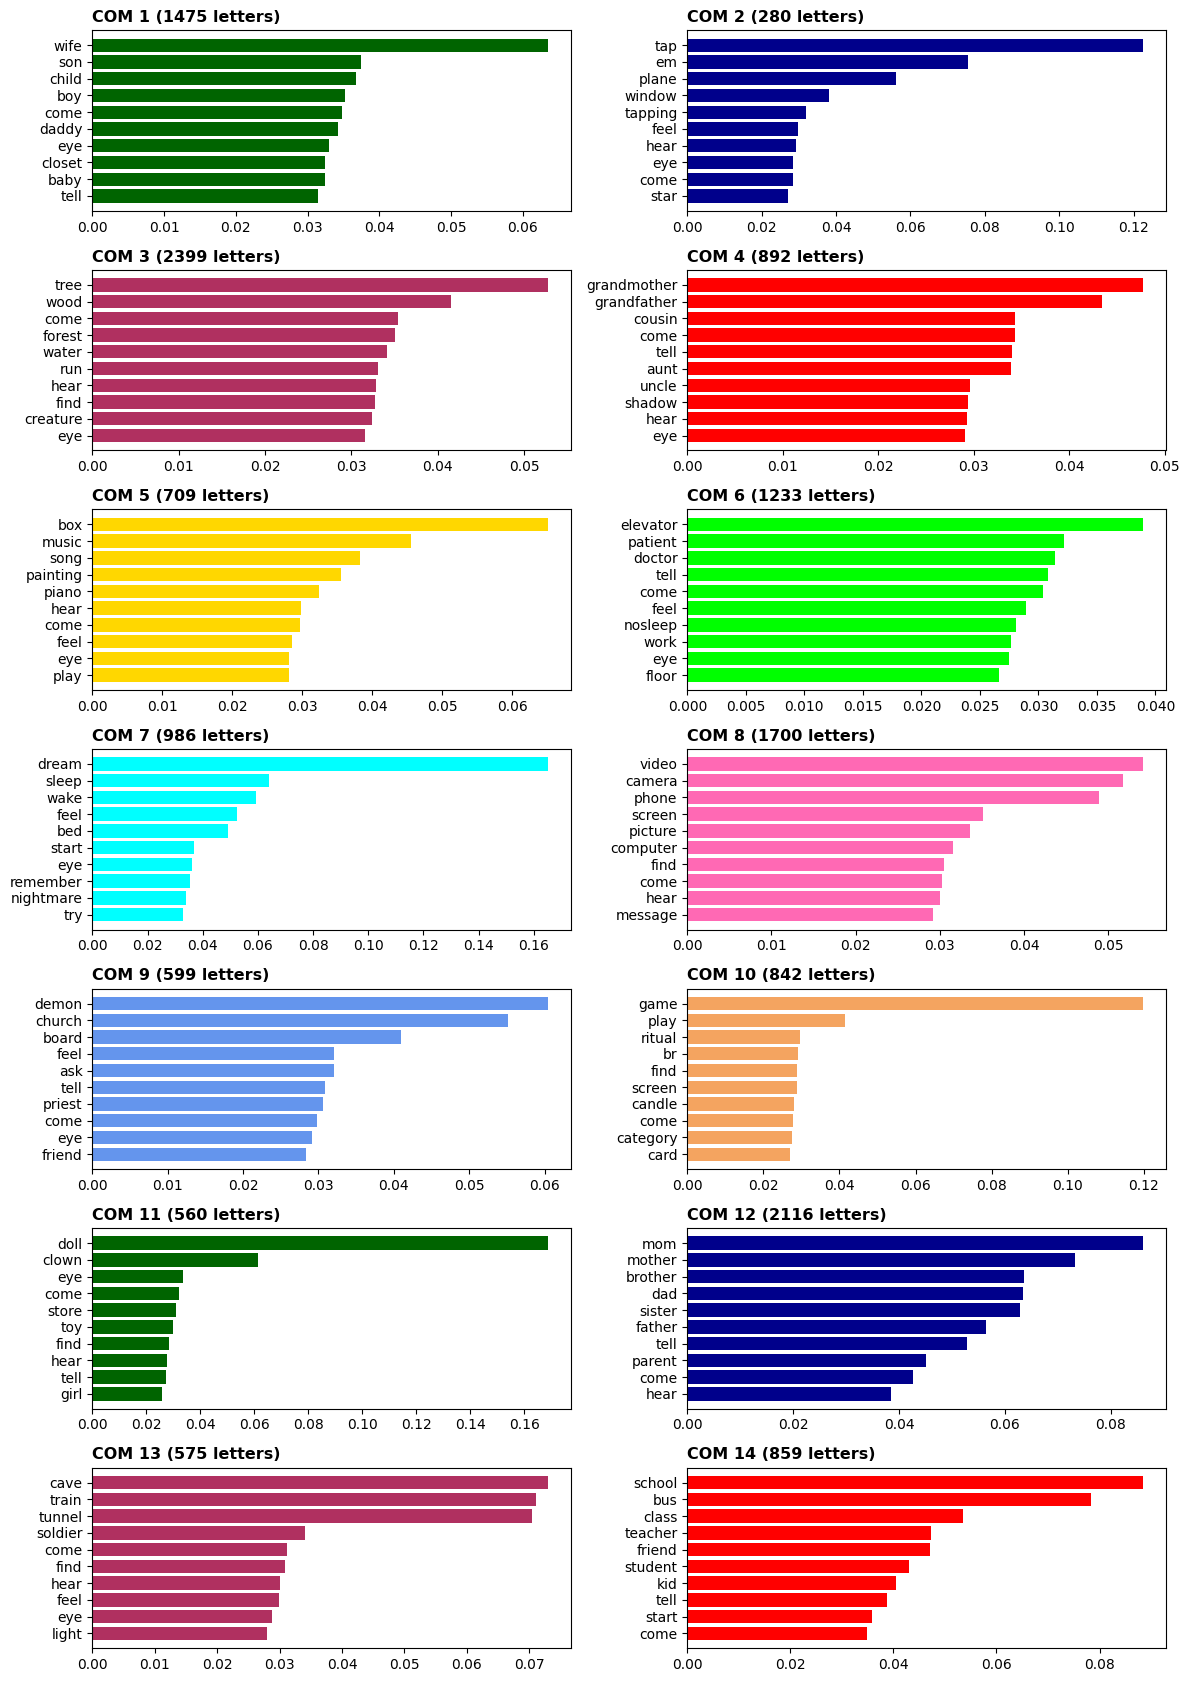
\includegraphics[width=0.8\textwidth]{tf_idf_topic_corpus.png}
    \caption{\small{Topic modelling réalisé grâce à un tf-idf sur un échantillon représentatif de mon corpus}}
\end{figure}


\end{document}
